% !TEX root=/home/tavant/these/manuscript/src/manuscript.tex




\chapter{Non-isothermal sheath model}
\label{ch-3}
% \renewcommand\leftmark{  \expandafter\MakeUppercase{ \chaptername\ \thechapter.\ Anisothermal sheath model}}
\headerchaptername{Non-isothermal sheath model}



\begin{Chabstract}
  
\emph{The work presented in this chapter has been published in  \citet{tavant2019}.}
\end{Chabstract}

\vspace{1ex}

\begin{Chabstract}
  
  In \Cref{ch-2}, discrepancies between the expected plasma-wall interaction quantities -- as the plasma potential drop through the sheath and the electron emission rate -- and the \ac{PIC} simulation results have been observed.
  In this chapter, we carry out a detailed analysis of the simulation results presented in \cref{ch-2}  in order to gain more insight on the plasma-wall interaction.
  We focus on a simplified simulation in order to isolate the plasma-wall interaction from the other phenomena.
  This new \ac{PIC} simulation is one-dimensional in space and three-dimensional in velocity (\acs{1D}-\acs{3V}), un-magnetized, and without electron emission.
  From this simplified simulation, we derived a non-isothermal sheath model, that describes well the kinetic simulations.
  We also extend the model to the case where ionization is self-consistent.

\end{Chabstract}

\minitoc

% !TEX root=/home/tavant/these/manuscript/src/manuscript.tex



\section{Insights for the PIC simulations}
\label{sec-insights}

As announced in \vref{sec-sheath_validation}, the sheath model of \vref{sec-sheath} uses two hypothesis\string:
\begin{itemize}
  \item Maxwellian electrons,
  \item Isothermal evolution of the electrons.
\end{itemize}

When collisions can be neglected, as it is usually assumed in the sheath, these two hypothesis are linked.
Indeed, the \ac{1D} Maxwellian distribution function expressed as the total energy is
\begin{equation} \label{eq-maxw_total}
  f(\ek, \phi) \propto \exp \lp \frac{\ek - \phi}{\Te}  \rp = \propto \exp \lp \frac{\ek}{\Te} \frac{-\phi}{\Te},
\end{equation}
where $\ek$ and $\Te$ are the electron kinetic energy and temperature expressed in Volt.
We can see in \cref{eq-maxw_total} that the spatial variation (due to the plasma potential $\phi$) only affect the amplitude of the distribution function, not its shape in the energy space.
Hence, the electron temperature is uniform, i.e. they are isotherm.
In addition, we find that $n_e \propto \exp (- \phi / \Te)$, which is the definition of Boltzmann electrons.

Hence, let see if this two aspects are respected in the \ac{2D} \ac{PIC}-\ac{MCC} simulation results

\subsection{Electron distribution function}

\begin{figure}[hbtp]
  \centering
  \includegraphics[width=\defaultwidth]{EEDF_2-eps-converted-to}
  \caption{Electron energy distribution function of the electrons ({\bf a}) in the bulk, in the three directions, and ({\bf b}) in the bulk and in the sheath}
  \label{fig-EEDF}
\end{figure}

Using the kinetic information of the PIC simulations, we present in \Cref{fig-EEDF} the mean electron energy probability functions (EEPF) in the case $\crover = 200\,\volt$.
\Cref{fig-EEDF}.{\bf a} shows the projections of the EEPF in the centre of the simulations along the three directions.
These projections are compared to the Maxwellian probability function of the same
kinetic temperature.
\Cref{fig-EEDF}.{\bf b} shows the total EEPF for both the bulk and the sheath populations.
 The sheath length is defined as the location where the ions reach the Bohm speed, which is about 0.4mm.
 
 We see in \cref{fig-EEDF}.{\bf a} that the electron distribution function is not Maxwellian.
 In particular the high energy tails are depleted.
 However, we can see that the electrons are rather isotropic, compared to \ac{1D} simulation \citep{sydorenko2006}.
 In order to evaluate the effect of the nonMaxwellian EEPF, we numerically integrate the EEPF from the PIC data using \vref{eq-ratedifinition_evdf}.
The results (not shown) do not differ significantly from the Maxwellian values of \vref{eq-seemaxw}.
Hence, we can conclude that even if the Maxwellian hypothesis is not respected in the
PIC simulations, it is not enough to explain the differences observed in \vref{fig-seeparamesMaxw}.


\Cref{fig-EEDF}.{\bf b} presents the EEPF for the bulk population as well as for the sheath population.
 We can see that the sheath population is colder than the population at the centre, which could explain the difference of \vref{fig-seeparamesMaxw}. 
 This effect is assessed in the next section.



 
% !TEX root=/home/tavant/these/manuscript/src/manuscript.tex

\section{Simplified 1D PIC simulations}
  \label{sec-1DPIC}

  We have seen in \cref{sec-insights} that the secondary electron emission is not responsible for the temperature radial profile.
  Hence, we neglect it in this section.
  The simulations are at low pressure, in which case  the electrons are non-local \cite{bernstein1954, godyak1993}.
  In low pressure bounded discharges, it is well-known that the EEDF is not Maxwellian in both capacitively coupled plasmas and inductively coupled plasmas \cite{mouchtouris2016, godyak2002, meige2006a, dominguez-vazquez2018}, in agreement with \cref{fig-EEDF}.

  The impact of non-Maxwellian EEDF on the electron flux to the wall has been studied by Kaganovich et al. \citep{kaganovich2000,kaganovich2007}.
  They showed that the electron kinetics at low pressure can significantly reduce the electron flux to the wall, in agreement with kinetic simulations.
  The main parameter determining the electron flux was found to be the electron scattering frequency.
  However, to our knowledge no fluid model describes the sheath with non-Maxwellian EEDF.

  The evolution of the electron temperature and the non-locality of the electrons in bounded plasmas has been studied in \citet{meige2006a}.
  The authors showed that the high energy tail of the \ac{EEDF} is depleted.
  They observed that the energy at which the depletion starts correspond to the local plasma potential related to the wall.
  Hence, we will use in this chapter similar physical conditions, in order to compare our results to their observations.

  \subsection{Description of the \acs{1D} simulations}

    We use a 1D PIC simulation of an argon plasma confined between two walls separated by a length $L=10$cm.
    The background pressure is varied between 0.05 and 10 mTorr.
    The direction of the simulation is $x$, and $y,z$ are perpendicular to the simulation domain.

    The same particle source model as in \ac{2D}\ac{PIC} of the \ac{HET} is used.
    In order to compensate the particle losses at the wall, we inject with a spatially uniform probability an electron-ion couple for every ion lost at the wall.
    This corresponds to the following ionization rate:
    \begin{equation}
      S_{iz} = \frac{1}{L} 2 \Gamma_e
    \end{equation}
    with $\Gamma_e$ the electron flux to the wall.
    A second model will be used later, with a self-consistent heating and ionization.

    Monte Carlo collisions (MCC) are still used, but we do not model the particle generation of the ionization process, but only the scattering and momentum transfer.
    As previously, Coulomb collisions are not included in the study as we are at low plasma density (at steady-state the electron density is around $n_e = 10^{15}$m$^{-3}$).

    To satisfy generally accepted accuracy conditions for the cell size and time step \citep{turner2013}, a time step of $3.7\cdot10^{-11}$\,s is used with a cell length of $1.7\cdot10^{-5}$\,m.
    This allows us to resolve properly the plasma frequency $\frac{2 \pi}{\omega_{pe}} = 3.5\cdot10^{-9} $\,s and the Debye length $\lambda_{De} = 3.10^{-4}$\,m.
    Around $300$ particles per cell are used for the simulations, and statistical convergence has been verified for both the cell length and the number of particles per cell.


    \begin{table}
      \centering
      \begin{tabular}{lll}  \toprule
        Parameter & Value & Unit  \\ \midrule
        Pressure $P$ & $0.05,0.1,0.5, 2, 10$ & mTorr\\
        Initial density & $1 .10^{15}$ & m$^{-3}$\\
        $\Te_{, inj}$& 5 & V\\
        Domain length $L$ & 10 & cm\\
        gas & Argon & -\\
        \bottomrule
      \end{tabular}
      \caption{Simulation parameters for the 1D PIC simulations.}
      \label{tab_1DPICParams}
    \end{table}


  \subsection{Simulation results of the \acs{1D} \acs{PIC} simulation} \label{subsec-1DPIC_results}

    \Cref{fig-PIC1} shows the results of the simulation with the parameters of \cref{tab_1DPICParams}.
    We only present in this section the result for neutral pressure $P=0.1$mTorr.
    The results obtained with different pressure show the same characteristics, and the effect of the pressure is further discussed in \cref{subsec-presurseffect}.
    
    \begin{figure}[!htb]
      \centering
      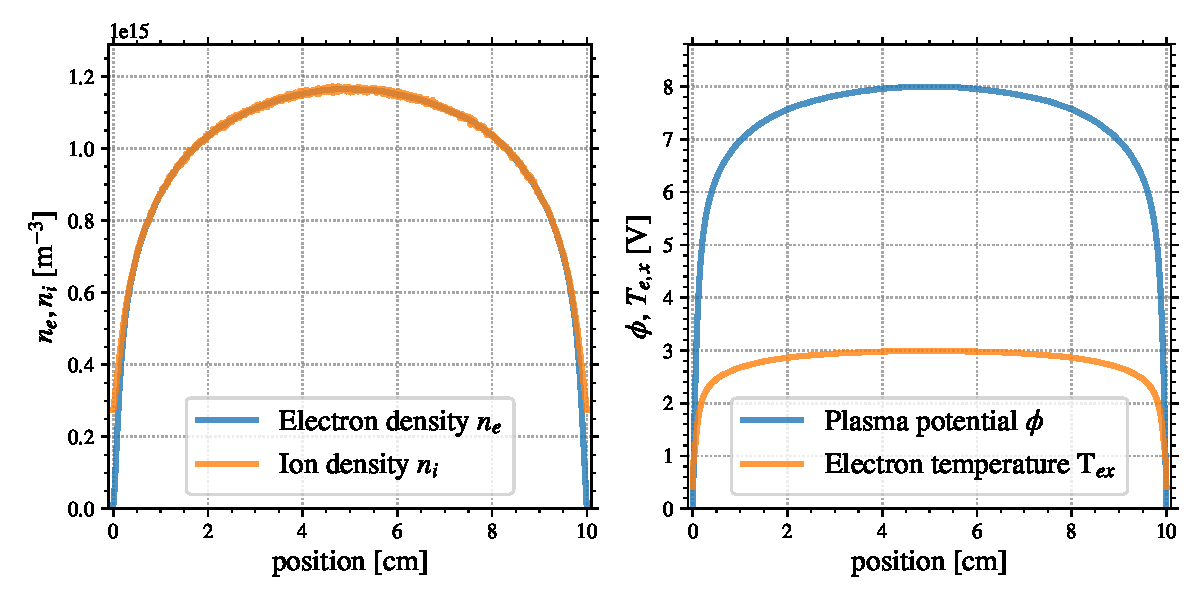
\includegraphics[width=\textwidth]{1D_PIC_summary.pdf}
      \caption{Profile of the electron and ion densities (left) and the plasma potential and electron temperature in the PIC simulation with the parameters of \cref{tab_1DPICParams}, with $P=0.1$mTorr.}
      \label{fig-PIC1}
    \end{figure}


    On the left-hand side we observe the electron and ion density profiles, while on the right the plasma potential and the electron temperature are shown.
    In \cref{fig-PIC1}, the electron and ion densities and the plasma potential feature the usual symmetric profiles with a pre-sheath and a sheath.
    However, while the electron temperature is almost constant in the plasma bulk at the center of the simulation domain, we observe a steep decrease in the sheath.
    The electron temperature gradient should affect the density profile in the sheath and the electron heat flux to the wall.

    \vspace{1em}
    For isotropic distribution functions, it is convenient to introduce the electron energy distribution function (EEDF) $f_{\epsilon}$ \citep{chabert2011}:
    \begin{equation}
    f_{\epsilon}(\epsilon) d\epsilon = 4 \pi v^2 f_e(\vec{v}) dv
    \end{equation}
    It is related to the electron energy probability function (EEPF) $f_{P}$ by
    \begin{equation}
    f_{P}(\epsilon) = \epsilon^{-1/2} f_{\epsilon}
    \end{equation}

    As the distribution function is anisotropic, and since the direction of interest is the $x$ direction, we focus here on $f_{P x}(\epsilon_x)$ the EEPF in the $x$ direction, with $\epsilon_x = \frac{m_e v_{e,x}^2}{2}$.


    \begin{figure}[!htbp]
      \centering
      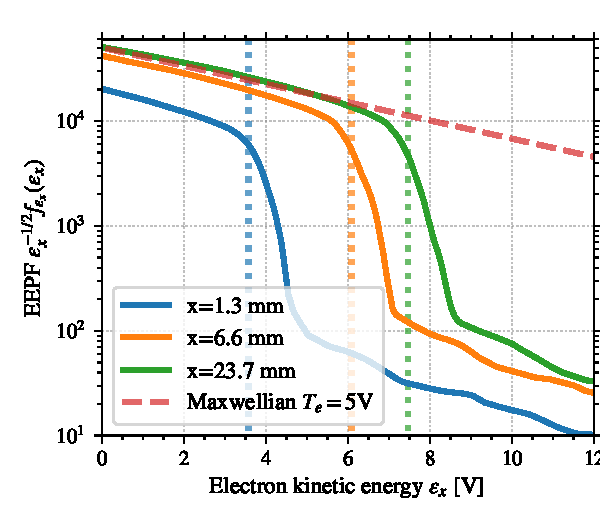
\includegraphics[width=\defaultwidth]{EVDFs.pdf}
      \caption{Electron energy probability function at different positions in the simulation: at $x=1.3,6.6$ and $23.7$ mm in blue, orange and green respectively. Also shown are the Maxwellian distribution of temperature $\Te=5\eV$ (red dashed line), as well as the local plasma potential relative to the wall $\dphi$ (dotted lines). }

      \label{fig-PIC2}
    \end{figure}

    \Cref{fig-PIC2} presents the EEPF measured in the PIC simulations at different positions.
    As the system is symmetric around x=5cm, the positions have been chosen arbitrarily in the left sheath, and their values correspond to the positions of the cell centers.
    We can see that the low energy population ($\ek < e \dphi$) is nearly Maxwellian, of temperature $\Te = 5\eV$ which is the injection temperature $\Te_{, inj}$.
    This population corresponds to the electrons confined by the sheath.
    However, the high energy tail ( $\ek > e\dphi$) is depleted due to the absorption at the wall \citep{meige2006a,kaganovich2007,lafleur2011}.
    This results in a  non-Maxwellian EEPF of temperature, defined with \cref{eq-defTe}, lower than $\Te_{, inj}$.
    The small population of electrons with very high energy corresponds to the electrons newly generated that have not yet reached the walls.



  \subsection{A model for the EVDF observed}
    \label{sec-twoTe}
    In order to describe the  EEPF seen in \cref{fig-PIC2}, it is possible to use a two-$\Te$ distribution \citep{lafleur2011,mouchtouris2016, zhang2016}:

    \begin{equation}
      f_{Px}(\ek_x) = A \ek_x^{1/2}
    \begin{cases}
      \exp( - \frac{\ek_x}{T_1} -  \frac{\epsilon_b }{T_2}) , \, \ek_x < \epsilon_b \\
      \exp( - \frac{\ek_x}{T_2} - \frac{\epsilon_b }{T_1} ) , \, \ek_x > \epsilon_b
    \end{cases}
    \end{equation}
    with $\epsilon_b$ the energy of the knee, $T_1$ and $T_2$ the two temperatures, and $A$ a normalization constant.
    In the case of absorption by the walls, we can assume that $\epsilon_b = \dphi$ as the absorption only occurs for the electrons of energy higher than $\dphi$.
    For the case of \cref{fig-PIC2}, we find $T_{1}=5$eV and $T_2=0.5$eV.
    This model is closer to the \ac{PIC} EEPF, but neglects the tails of newly generated electrons of high temperature, as we can see if in \Cref{fig-PIC3}.


    \begin{figure}[!hbt]
      \centering
      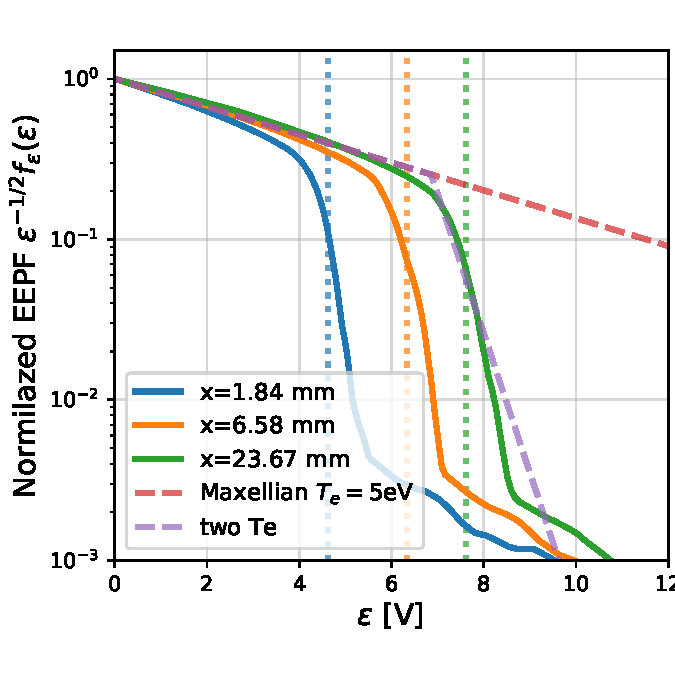
\includegraphics[width=\defaultwidth]{EVDFs_and2Te}
      \caption{Electron energy probability function at different positions in the simulation, as in \cref{fig-PIC2}, but overlaid with a 2-temperature distribution function.}
      \label{fig-PIC3}
    \end{figure}

    In the next section, we investigate a way of taking into account this non-local kinetic phenomenon in a fluid model.

% !TEX root=/home/tavant/these/manuscript/src/manuscript.tex

\section{Collisionless kinetic model and polytropic state law}
  \label{sec-kinetic}


  The previous section showed that in the \ac{1D} \ac{PIC} simulations the electrons are not Maxwellian, similarly to the \ac{2D} results.
  In this section, we use the 1D kinetic equation in order to highlight the important phenomena needed to describe the sheath.
  
  \subsection{Vlasov equation for the sheath}

    Because the sheath is thin and the neutral pressure is low, we neglect the collisions in the sheath, so that we only need to solve Vlasov's equation.
    The stationary 1D-3V Vlasov equation for the EVDF reads\string:
    \begin{equation}\label{eq-vlasov}
      v_x \cdot \partial_x f_e \vec{e}_x + \frac{e}{m_e} \nabla \phi \cdot \nabla_v f_e = 0,
    \end{equation}
    Since the electrostatic potential depends only on $x$, \cref{eq-vlasov} becomes,
    \begin{equation}
    v_x \partial_x f_e +  \frac{e}{m_e}\partial_x\phi \partial_{v_x} f_e = 0
    \label{eq-vlasov1D}
    \end{equation}
    The variables $v_y$ and $v_z$ do not play any role, such that they can be hold constant, and we can solve \cref{eq-vlasov1D} with $f_e$ as a function of $x$ and $v_x$ only.

    In order to solve \cref{eq-vlasov1D} in the sheath,  we use the following boundary conditions\string:
      \begin{enumerate}
    \item At the plasma sheath boundary ($x=x_s$) the EEDF is imposed\string:
    \begin{equation}
    f_e(x_s, v_x) = f_0(v_x),
    \label{eq-plasma_BC}
    \end{equation}
    \item At the wall ($x=x_w$) the particles are absorbed, such that
    \begin{equation}
    f(x_w, v_x<0) = 0
    \label{eq-wall_BC}
    \end{equation}
    \end{enumerate}

    The partial derivative equation (\ref{eq-vlasov1D}) can be solved by the method of the characteristics. We introduce the function $\gamma(x)$ such that
    \begin{equation}
      \frac{df_e(x,\gamma(x))}{dx} = \partial_x f_e + \gamma' \partial_{v_x} f_e = 0
    \end{equation}
    Combining this equation with \cref{eq-vlasov1D} for $v_x = \gamma(x)$,
    \begin{equation}
      \label{eq-char}
      \left( \frac{e\phi'}{m_e} - \gamma \gamma' \right) \partial_{v_x} f_e = 0
    \end{equation}
    In general $\partial_{v_x} f_e \neq 0$ such that $(e\phi'/m_e - \gamma\gamma')$ can be integrated
    \begin{equation}
      \frac{\gamma(x)^2}{2} - \frac{e\phi(x)}{m_e} = \frac{\gamma(x_s)^2}{2} - \frac{e\phi_s}{m_e}
    \end{equation}
    Since the EVDF is conserved along the contour $\gamma$,
    \begin{equation}
      f_e(x,\gamma(x)) = f_e(x_s, \gamma(x_s))
    \end{equation}
    and
    \begin{equation}
      \gamma(x_s) = \left[ \gamma(x)^2 - \frac{2e(\phi(x) - \phi_s)}{m_e} \right]^{1/2}
    \end{equation}
    with $\phi_s$ the plasma potential at the sheath edge.
    Using \cref{eq-plasma_BC},
    \begin{equation}
      \label{eq-sol}
      f_e(x,v) = f_0\left( \left[ v^2 - \frac{2e(\phi(x) - \phi_s)}{m_e} \right]^{1/2}\right)
    \end{equation}
    Condition (\ref{eq-wall_BC}) yields a condition on $f_0$\string:
    \begin{equation}
      \label{eq-trunc}
      \text{for all } v > \left( \frac{2e\phi_s}{m_e} \right)^{1/2}, f_0(v) = 0
    \end{equation}
    
    This simple collisionless model explains rigorously how the tail of the EVDF is cut by the wall absorption.
    This asymmetry of the \ac{EVDF} could press us to separate the electrons into the population going toward the wall and the one going away from the wall.
    \Cref{fig-EVDFpm} shows the EEPF of the electron going toward and from the wall.
    We can see that there is only a small difference between the  EEPF of the two populations.
    Indeed, as the domain is symmetric and bounded in the two directions, the population coming toward the wall is also depleted by the opposite wall.
    Hence in the following, we will neglect this asymmetry due to the wall.


    \begin{figure}[!hbt]
      \centering
      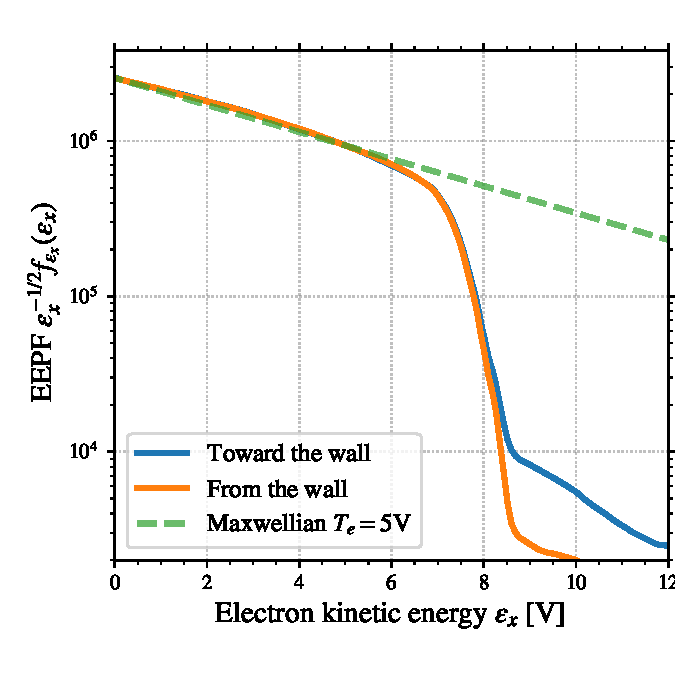
\includegraphics[width=\defaultwidth]{EVDFpm.pdf}
      \caption{EEPF measured in the PIC simulations of the electrons going toward and from the wall at $x=23.7mm$. The green dashed line corresponds to a Maxwellian distribution of 5$\eV$.}
      \label{fig-EVDFpm}
    \end{figure}

    \begin{figure}[!hbt]
      \centering
      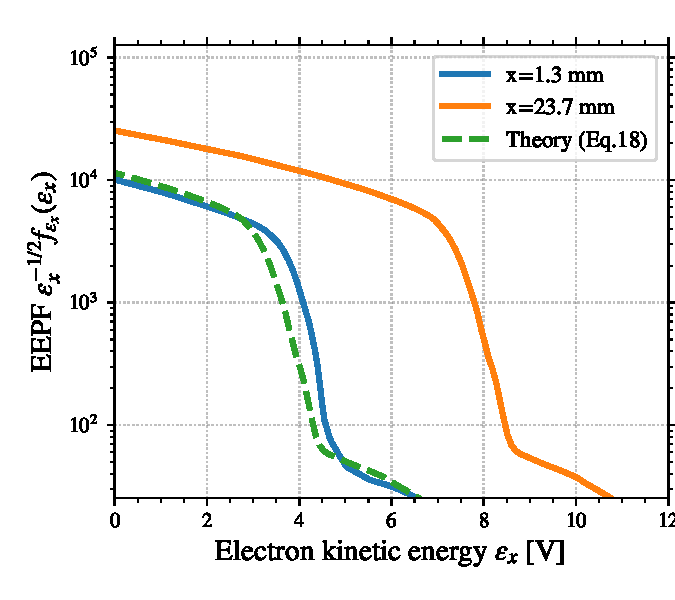
\includegraphics[width=\defaultwidth]{EVDFshift.pdf}
      \caption{Evolution of the EEPF between 1.3mm (in blue) and 23.7mm (in orange) from the wall. Is overlaid (in dashed green) the expected  EEPF at $x=1.3$mm using the EEPF at $x=23.7$mm and the potential difference in \cref{eq-sol}. }
      \label{fig-PICEEPF}
    \end{figure}

    \Cref{fig-PICEEPF} compares the EEPF from \cref{eq-sol} with the \ac{PIC} simulations between the position $x=1.3$\,mm and $x=23.7$\,mm.
    The plasma potential reads $\phi(x=1.3\,{\rm mm})=4.1$\,V and  $\phi(x=23.7\,{\rm mm})=7.7$\,V.
    We can observe a very good agreement between the actual evolution of the EEPF measured in the simulations and the prediction of \cref{eq-sol}.
    This confirms the possibility to neglect the collisions in the sheath.

  \subsection{Polytropic state law for the electrons}

    The evolution of a two-$\Te$ EEDF  in a collisionless potential drop has been studied by \citet{zhang2016}.
    The authors have shown that the evolution of the electron population can be described using a polytropic index $\gamma$, such that\string:
    \begin{equation}
      \label{eq-poly}
      \nabla_x \left( p_{e,x}(x) n_e(x)^{-\gamma} \right)= 0
    \end{equation}
    with $p_{e,x}$ the electron pressure.
    The value of $\gamma$ is related to the two temperatures $T_1$ and $T_2$, and for $T_1 > T_2$, we have $\gamma > 1 $.




    \begin{figure}[!htb]
      \centering
      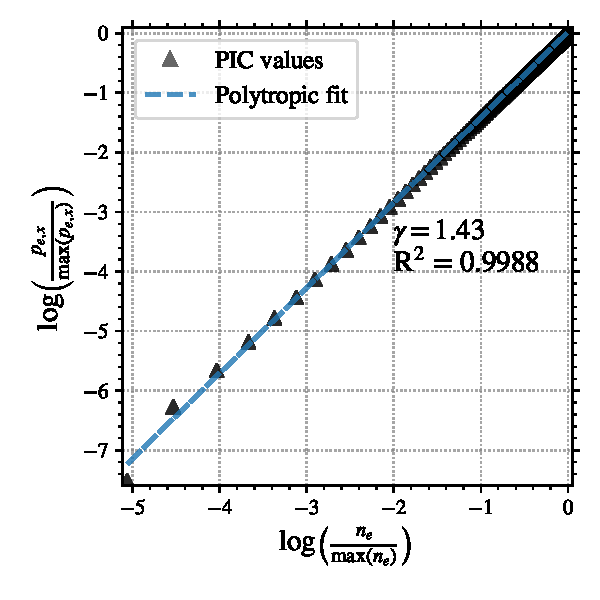
\includegraphics[width =\defaultwidth]{Polytropic.pdf}
      \caption{Electron pressure as a function of the electron density observed in the PIC simulations of \cref{fig-PIC1} (black markers), and the linear fit (blue dotted line) in order to determine $\gamma$.}
      \label{fig-polyFit}
    \end{figure}

    \Cref{fig-polyFit} shows the PIC simulation results presented in \cref{fig-PIC1} in log scale.
    Each marker represents one cell of the PIC simulation.
    Overlaid is a linear regression which slope is the polytropic index $\gamma$.
    The regression is conducted over the whole simulation domain.
    We can see that the linear regression fits the simulation results with a very good agreement (R$^2$ = 0.999).
    The value $\gamma = 1.43$ is significantly higher than the isothermal case ($\gamma_{\rm isothermal} = 1$).
    Interestingly, while the polytropic law observed in \citet{zhang2016} was only for a collisionless evolution, here the polytropic law is observed in both the collisionless sheath and the weakly collisional plasma region.

    The polytropic law of \cref{eq-poly} can be used in order to close the fluid equation without the isothermal hypothesis.
    The non-isothermal fluid model for the sheath is the subject of \cref{sec-fluid}.
    A polytropic index for the ions has already been proposed in order to link the ions kinetics and the fluid parameters \citep{kuhn2006,jelic2007}.
    The approach here is essentially the same but applied to the electrons.


  \subsection{Evolution of the polytropic index}
    \label{subsec-presurseffect}
    We investigate the effect of the neutral pressure on the polytropic index $\gamma$ for the 5 pressure conditions of \cref{tab_1DPICParams}.
    We recall that the electron elastic scattering and momentum transfer are modeled, while the ionization and the heating are not self-consistent, but they are similar to the \ac{2D} \ac{PIC} models of \cref{ch-2}.
    \Cref{fig-p} presents the evolution of $\gamma$ as a function of the pressure.
    We can see that the polytropic index decreases from 1.7 to 1.4 as the pressure increases from 0.05 to 10 mTorr.
    This is in agreement with the fact that the high energy electron population is mostly replenished by the electron-neutral scattering, in agreement with \citet{kaganovich2007}.
    Increasing the collisions while keeping the other parameters constant provides more electrons to the high energy tail, hence reducing the polytropic index, as observed by \citet{zhang2016}.

    \begin{figure}[!htb]
      \centering
      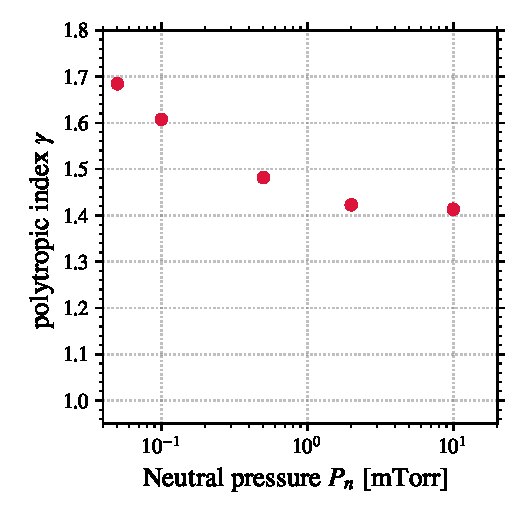
\includegraphics[width=\defaultwidth]{pressur_effectLog.pdf}
      \caption{Effect of the background neutral pressure over the polytropic index $\gamma$ in the \acs{1D} \acs{PIC} simulations, under the conditions of \cref{tab_1DPICParams}. As a reminder, the isothermal case corresponds to $\gamma=1$.}
      \label{fig-p}
    \end{figure}

    Other parameters are also expected to modify $\gamma$.
    For instance the size of the simulation, the electron mean energy, and the nature of the gas.

  \subsection{Coulomb collision and possible improvements}
  
    In the \ac{PIC} simulations, the Coulomb collisions (electron-electron, electron-ion, and ion-ion) are not modeled.
    However, they are known to modify the distribution function.
    More precisely, they isotropize the distribution and tend toward a Maxwellian \citep{bhatnagar1954,sydorenko2006b}.
    
     Using the density $n_e=\sn{1}{15}\,\per\meter\cubed$ and the electron temperature $\Te=3\,\volt$ we find the electron-electron Coulomb collision at 90$^{\circ}$ \citep{lieberman2005,chen2006}
     \begin{equation} \label{eq-nu_Coulomb}
       \nu_{90} = 15 \,\kilo\hertz
     \end{equation}
     which is significantly smaller than the electron-neutral scattering frequency.
     However, it is known that the Coulomb collisions cross-section is highly dependent on the electron velocity.
     
     \Cref{fig-mfp_coulomb} shows the evolution of the mean free path for the electron-electron Coulomb collision $l_{CC} = v_e/\nu_{90}$.
     We can see that it is of the order of the domain size ($L=10\,\centi\meter$) only for very low energy.
     \begin{figure}[!hbt]
       \centering
       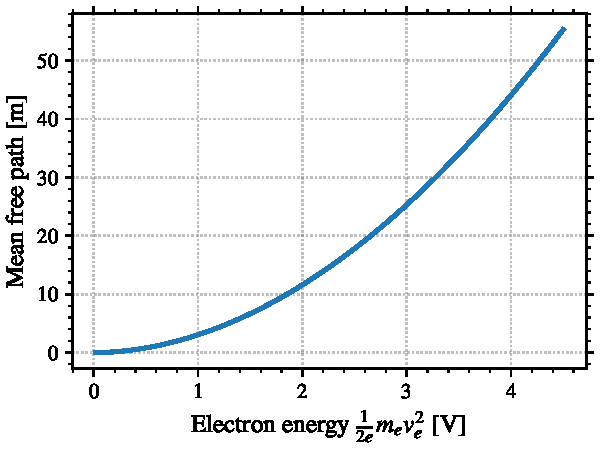
\includegraphics[width=\defaultwidth]{Coulomb_collision_meanfreepath_zoom}
       \caption{Mean free paths of the Coulomb collision as a function of the electron energy.}
       \label{fig-mfp_coulomb}
     \end{figure}
     \inlinenote{Anne: Le e est pour la conversion en V}
     On the other hand, the collision frequency for small angle is higher.
     In \citet{sydorenko2006b}, the authors showed that under some conditions, the Coulomb collisions can modify the simulation results by a few tens of percent.
     Hence, the impact of the small angle Coulomb collisions on the distribution functions should be asserted in future work.
     Modeling the Coulomb collision in \ac{PIC} simulations currently require a different model than the \ac{MCC} algorithm, thus requires more time to be implemented and tested before being used.

     

% !TEX root=/home/tavant/these/manuscript/src/manuscript.tex

\section{Non-isothermal  fluid model }
\label{sec-fluid}

We have seen in \cref{sec-kinetic} that the polytropic law presented in \cref{eq-poly} can be used to describe the evolution of the electron temperature, hence closing the fluid equations.
Provided that the electron pressure is $p_e = e n_e \Te$, assuming the sheath collisionless, and neglecting the electron mean velocity compared to the thermal velocity, the electron momentum conservation
\begin{equation}
\label{eq-elec_mom}
 \nabla (n_e \Te) + n_e \nabla \phi = 0
\end{equation}
results in
\begin{equation}
  \label{eq-momentum}
  \nabla \Te = - \frac{\gamma - 1}{\gamma} \nabla \phi
\end{equation}
Integrating \cref{eq-elec_mom} from the sheath edge, the electron density is hence:
\begin{equation}
  \label{eq-ne}
  n_e(\phi) = n_0 \left[ 1 + \frac{(\gamma - 1) (\phi - \phi_0)}{\gamma \Te_0}  \right]^{\frac{1}{\gamma - 1}}
\end{equation}
with the subscript $0$ corresponds to the sheath edge.
In \cref{eq-ne}, we need to have $\gamma$ strictly greater than one.
For $\gamma=1$, we find the usual Boltzmann electrons:
\begin{equation}
  n_e(\phi) = n_0 \exp( - \frac{ (\phi - \phi_0)}{\Te})
\end{equation}
corresponding to the usual isothermal model.

\subsection{Comparison with the PIC simulations}
\label{sec-fluidPIC}
The PIC simulations of \cref{sec-1DPIC} can be modeled using a 1D low pressure fluid model with collisionless ions.
We use the solver described in \citet{riemann2005}, modified to take into account the new electron closure.
We simply need to add one equation for the temperature, and the ionization source term is fixed constant in space.

Using the normalized variables and parameters:
\begin{align}
\lambda &= \frac{S_{iz} L}{c_s}, &\Phi&=-\frac{e \phi}{\Te_{, c}}, &u &= \frac{v_i}{c_s}\\
n &= \frac{n_i}{n_{e,c}}, &\chi&=\lambda \frac{x}{L}, &\epsilon &= \lambda \frac{\lambda_{De}}{L}\\
\end{align}
with $\Te_{,c}, n_{e,c}$ the electron temperature and density at the center, $c_s= \sqrt{\frac{\Te_{,c}}{m_i}}$ the ion sound speed, $v_i, n_i$ the ion speed and density, and $S_{iz}$ the ionization frequency, we can write the set of equations representing the plasma as\citep{riemann2005}:



\begin{equation}
  \label{eqs-fluid}
  \begin{cases}
    d_{\chi} (n u ) &= \lambda\\
    d_{\chi} (u) &= \frac{d_{\chi} (\phi)}{u} - \frac{\lambda}{n}\\
    d_{\chi}^2 (\Phi) &= \frac{(n - n_e)}{\epsilon^2}\\
    S_{iz} &= cst \\
    n_{e} &= \left[ 1 + \frac{(\gamma - 1) \Phi }{\gamma}  \right]^{\frac{1}{\gamma - 1}}
\end{cases}
\end{equation}

Starting from the center, and using the results of the PIC simulations to determine $\gamma$, we can use the system of \cref{eqs-fluid} to compute the profile of every variable.
The plasma potential is self consistently computed from an arbitrary value at the center.
It is then shifted to set the wall potential to 0V.
The integration uses the \nth{4} order Runge-Kutta integration scheme of the python package \texttt{scipy}.


\begin{figure}[!htbp]
  \centering
  % 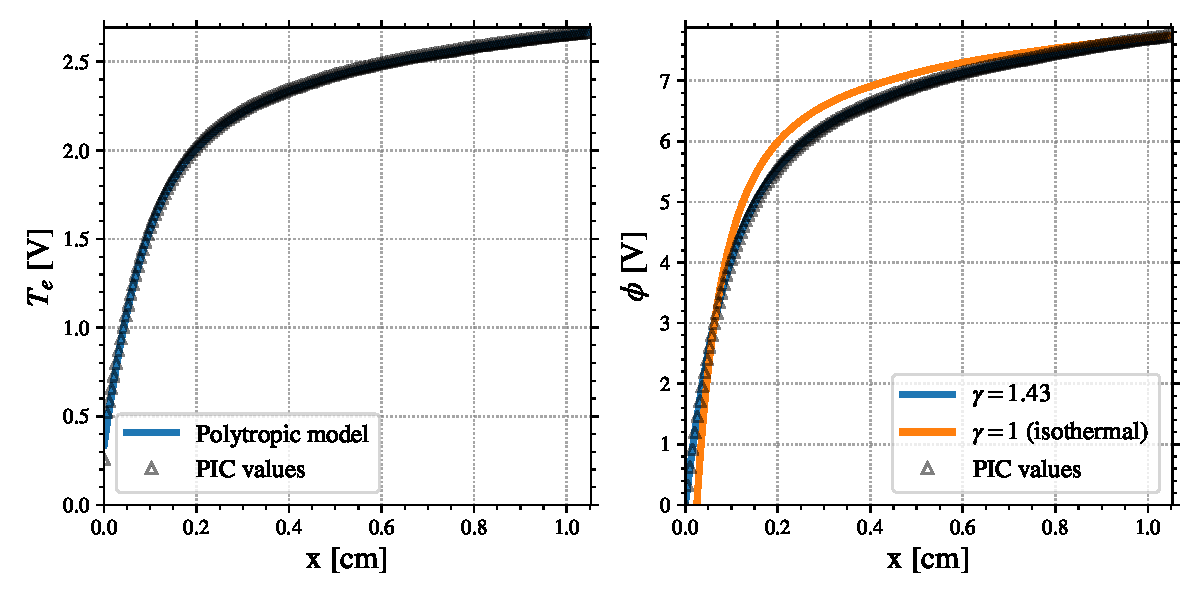
\includegraphics[width = 0.7\textwidth]{figures/sheathModel.pdf}
  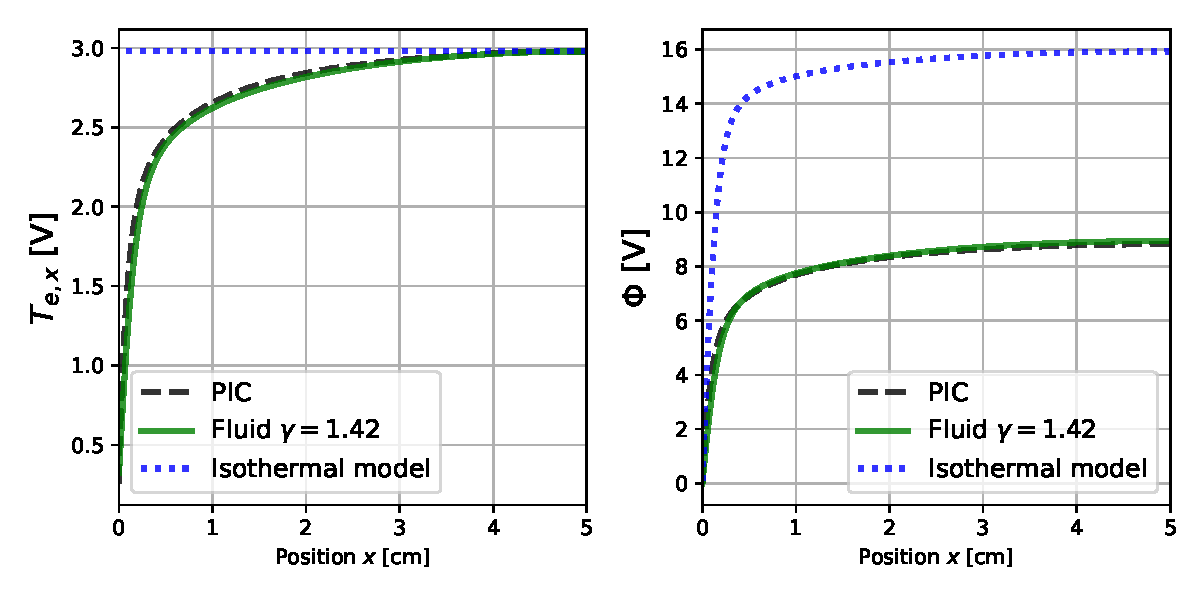
\includegraphics[width = 0.7\textwidth]{FluidComparison.pdf}
  \caption{Comparison of the electron temperature and plasma potential measured in the PIC simulation with the prediction of the polytropic model with $\gamma = 1.42$.}
  \label{fig-comp}
\end{figure}

\Cref{fig-comp} shows the comparison of the electron temperature and the plasma potential with the resolution of the set of \cref{eqs-fluid}.
We can see a very good agreement between the model and the PIC simulations.


\subsection{Modified Bohm criterion}
The Bohm criterion expresses a necessary condition on the ion velocity at the sheath edge for the formation of a stationary sheath \citep{riemann1991}.
As discussed in the appendix, it is possible to derive a modified Bohm criterion for the polytropic electrons:
\begin{equation}
  \mathcal{M}^2 = \left( \frac{u_0}{c_s} \right)^2 \geq \gamma
\end{equation}
with $\mathcal{M}$ the Mach number, $u_0$ the ion mean velocity at the sheath edge and $c_s=\left( \frac{e \Te_0}{m_i} \right)^{1/2}$ the ion acoustic velocity at the sheath edge. The derivation of this modified Bohm criterion is analogous to the isothermal case.
In the same way as for the isothermal Debye sheath, we assume that the sheath criterion is saturated:
\begin{equation}
  \label{eq-saturation}
  \mathcal{M}^2 = \gamma.
\end{equation}

In addition, the ion flux at the wall is equal to the flux at the sheath edge:
\begin{equation}
  \label{eq-gi}
  \Gamma_i = n_0 \sqrt{\frac{\gamma e \Te_0}{m_i}}
\end{equation}

\subsection{Plasma potential drop to the wall}
The electron flux at the wall is the thermal flux:
\begin{equation}
  \label{eq-geki}
  \Gamma_e = \int_0^{+\infty} v f_e(x=x_w,v) dv
\end{equation}
Using the model of two-Te EEDF described in \ref{sec-twoTe}, we obtain
\begin{equation}
  \label{eq-ge}
  \Gamma_e = \frac{1}{4} n_{e,w} \bar{v}_w
\end{equation}
with $n_{e,w}$ the electron density at the wall, and $\bar{v}_w = \sqrt{\frac{8 e\Te_{,w}}{\pi m_e}}$ the mean electron speed at the wall, using $\Te_{,w}$ the electron temperature at the wall.
Using \cref{eq-momentum}, we have:
\begin{equation}
  \label{eq-tew}
  \Te_{,w} = \Te_0 \left(  1 - \frac{\gamma -1}{\gamma}\frac{\dphi_0}{\Te_0}  \right)
\end{equation}
with $\dphi_0$ the potential drop between the sheath edge and the wall.
Using the current equality: $\Gamma_i = \Gamma_e$ at the wall we find with \cref{eq-gi,eq-ge,eq-tew}:
\begin{equation}\label{eq-sheath}
  \left[ 1 +\frac{\gamma -1}{\gamma} \frac{ \dphi_0}{ \Te_0}  \right]^{\frac{1}{\gamma - 1}} \sqrt{1 - \frac{\gamma -1}{\gamma}\frac{\dphi_0}{\Te_0}} = \sqrt{\frac{4 \gamma \pi m_e}{m_i}}
\end{equation}

\Cref{eq-sheath} cannot be solved analytically, but it can be solved numerically.
We use the function \texttt{fsolve} from python package \texttt{scipy.optimize} to plot the solution of \cref{eq-sheath} in \cref{fig-dphinorm}.
Meanwhile, we estimate $\frac{\Delta \phi_0}{\Te_0}$ using the fluid model of \cref{sec-fluid} by reading the potential at the position for which the ions reach the modified Bohm velocity.
The small difference between the solution of \cref{eq-sheath} and the fluid solution is due to the presence of ionization in the sheath.

\begin{figure}[!htbp]
  \centering
  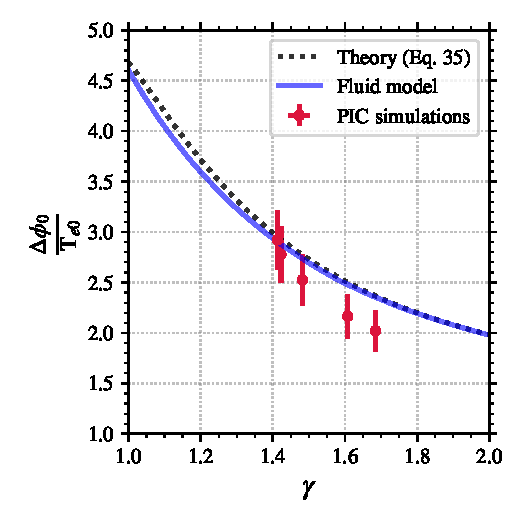
\includegraphics[width=\defaultwidth]{phinorm_theoryAndPIC2.pdf}
  \caption{Evolution of the potential drop normalized to the electron temperature as a function of the polytropic index $\gamma$ from the theory of \cref{eq-sheath}, from the fluid model of \cref{sec-fluidPIC} and from the PIC simulations results (the same cases as in \cref{fig-p}). Errors correspond to 10\% . }
  \label{fig-dphinorm}
\end{figure}


\Cref{fig-dphinorm} shows the evolution of normalized plasma potential drop to the wall $\frac{\dphi_0}{\Te_0}$ as a function of $\gamma$.
{  Error bars indicate an uncertainty of 10\%.
This uncertainty value corresponds to an aggregation of the numerical fluctuation of the PIC simulation (that decreases when more particles per cell are used), and the estimation of the sheath edge position.
A more accurate estimation of these uncertainties would require a dedicated study with many additional simulations, hence we choose the reasonable value of 10\% \citep{turner2013}.}
We can see that in the limit where $\gamma \rightarrow 1$, we find with \cref{eq-sheath} the usual isothermal value $\frac{\dphi_0}{\Te_0}  \simeq 4.68$ for argon.
The value observed in the fluid model is very close to the results of \cref{eq-sheath}.
This is due to the very small size of the sheath, as seen in \cref{fig-PIC1}.
When $\gamma$ increases, $\frac{\dphi_0}{\Te_0}$ decreases significantly.
The decrease of $\dphi_0$ is consistent with the depletion of the high energy tail of the electrons, as the plasma needs less screening of the electrons in order to stay quasi-neutral.

\Cref{fig-dphinorm} also presents the potential drop measured in the same PIC simulations as presented in \cref{fig-p}.
The error bars correspond to an estimate of the aggregation of the uncertainties from the PIC simulation and the averages.
The sheath edge is defined using the modified Bohm criterion (\cref{eq-saturation}), as for the fluid model.
We can see a very good agreement with the theories.
The trend of decreasing potential drop with increasing $\gamma$ is clearly observed, and the values agree within about $10\%$.
This is significantly more accurate than the $50$\% discrepancy with respect to the isothermal model.\\

The solutions of \cref{eq-sheath} can be fitted between $\gamma = 1$ and $\gamma = 2$ with a good precision ($R^2 = 0.98$) by:
\begin{equation}
  \label{eq-fit}
  \frac{\dphi_0}{\Te_0} = 0.7 + \frac{4.1}{\gamma^{1.7}}
\end{equation}
%Although the expression of \cref{eq-fit} has no physical origin.

\subsection{Power losses at the wall}

As expressed in the previous section, the electron flux to the wall is equal to the ion flux:
\begin{equation}
  \Gamma_e = \Gamma_i =  n_0 \sqrt{\frac{\gamma e \Te_0}{m_i}}
\end{equation}
with $n_{e,0}$ and $\Te_0$ the electron density and temperature at the sheath edge.
Following the two-$\Te$ EEDF as described in \cref{sec-kinetic}, the electron energy flux to the wall is a thermal flux from a Maxwellian distribution function of temperature  $\Te_w$.
Hence it reads \cite{charbertBook}:
\begin{equation}
  \label{eq-maxflux}
  Q_e = \Gamma_e 2 \Te_{w}
\end{equation}

Using \cref{eq-tew}, we obtain
\begin{equation}
  \label{eq-meanE}
  \frac{Q_e}{\Gamma_e} =  2 \Te_0 \left[1 - \frac{(\gamma - 1)}{\gamma} \frac{\dphi_0}{\Te_0} \right]
\end{equation}
with $\frac{\dphi_0}{\Te_0}$ calculated from either \cref{eq-sheath} or \cref{eq-fit}.
From \cref{eq-meanE} we see that in the isothermal limit we find the usual $2 \Te$ mean energy by electron leaving the plasma.
However, for $\gamma > 1$, the mean energy by electron decreases.


\begin{figure}[!htbp]
  \centering
  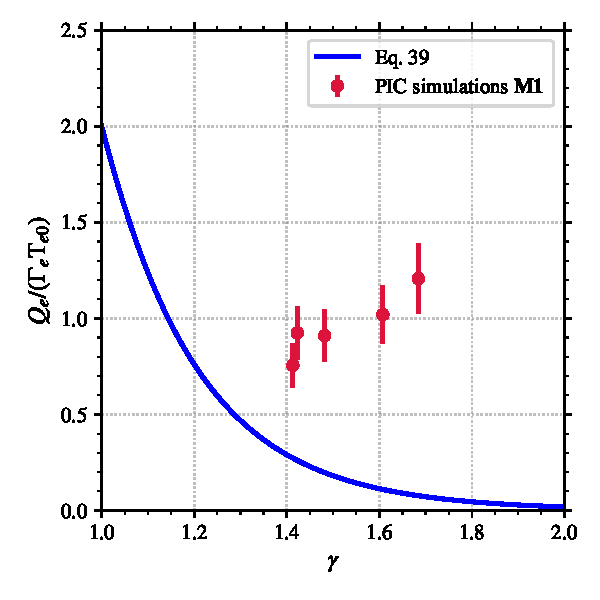
\includegraphics[width=\defaultwidth]{meanelectronenergy_PIC.pdf}
  \caption{Evolution of the mean energy per electron leaving the plasma at the wall normalized to the electron temperature at the sheath edge as a function of the polytropic index $\gamma$ from the theory of \cref{eq-meanE}. The simulation result (marker) corresponds to the model \M1. }
  \label{fig-avE}
\end{figure}

\Cref{fig-avE} shows the evolution of the average energy of electrons leaving the plasma at the wall normalized to the electron temperature in the plasma bulk from \cref{eq-meanE}.
We can see that the ratio is significantly lower than the isothermal value $\frac{Q_e}{\Gamma_e} = 2 \Te_0$ when $\gamma > 1$.
Overlaid in \cref{fig-avE} are the PIC simulation results.
We can see that the PIC results are lower than the isothermal value, but do not agree well with \cref{eq-meanE}.
The discrepancy could be due to the two-Te hypothesis used in \cref{eq-maxflux}.
Indeed, we can see in \cref{fig-EVDFpm} that there is a small population of high energy electrons.
This population is not big enough to modify the electron flux to the wall, hence the potential drop \citep{demidov2005}, but may increase the mean energy of electron leaving the plasma.
{  We tested the hypothesis for one case ($P_n=2$ mTorr).
Once the steady state was reached, we stopped generating the electron-ion couples.
We observed that during a transition time of around $0.74 \mu$s, the mean energy per electron decreased significantly from $0.9$~V to $0.3$~V, while the electron flux to the wall $\Gamma_e$ and the electron temperature $\Te_{, 0}$ was not yet affected.
This is more consistent with \cref{eq-meanE} and seems to confirm the hypothesis, but more investigations on the heat flux are needed.
  }

% !TEX root=/home/tavant/these/manuscript/src/manuscript.tex

\section{Realistic heating and ionization}
  \label{sec-realistic_1D}
  In the study of \cref{{sec-1DPIC}}, the ionization and the heating mechanism are not physical, but allowed us to obtain a steady state as in the simulations of \cref{ch-1}.

  Hence, we study the impact of the wall absorption in a case of self-consistent heating and ionization.
  The electrons are heated "inductively" with a radio-frequency (RF) electric field in the direction normal to the simulation grid \cite{meige2006a, lucken2018, turner1993}.
  The electrons are heated in the $y$ direction, and momentum is transferred to the $x$ and $z$ axis via electron-neutral collisions.
  The heating electric field $\vec{E_{rf}} = E_{rf} \vec{e_y}$ is independent of $x$ in the simulation domain, its frequency is $13.56$\,MHz, and its amplitude is adjusted in order to obtain the desired absorbed power $P_{abs} = < \vec{J_e} \cdot  \vec{E_{rf}}>$.
  


  \begin{table}[!htbp]
    \centering
    \begin{tabular}{c | c | c}
      Parameter & value & unit \\ \hline
      Pressure & $0.1$ & mTorr\\
      $P_{abs}$ & $0.25$ & W/m$^{-3}$\\
      Length $L$&10&cm\\
    \end{tabular}
    \caption{Input parameters for the simulation using the self-consistent model.}
    \label{tab-PIC2}
  \end{table}

  \begin{figure}[!htbp]
    \center
    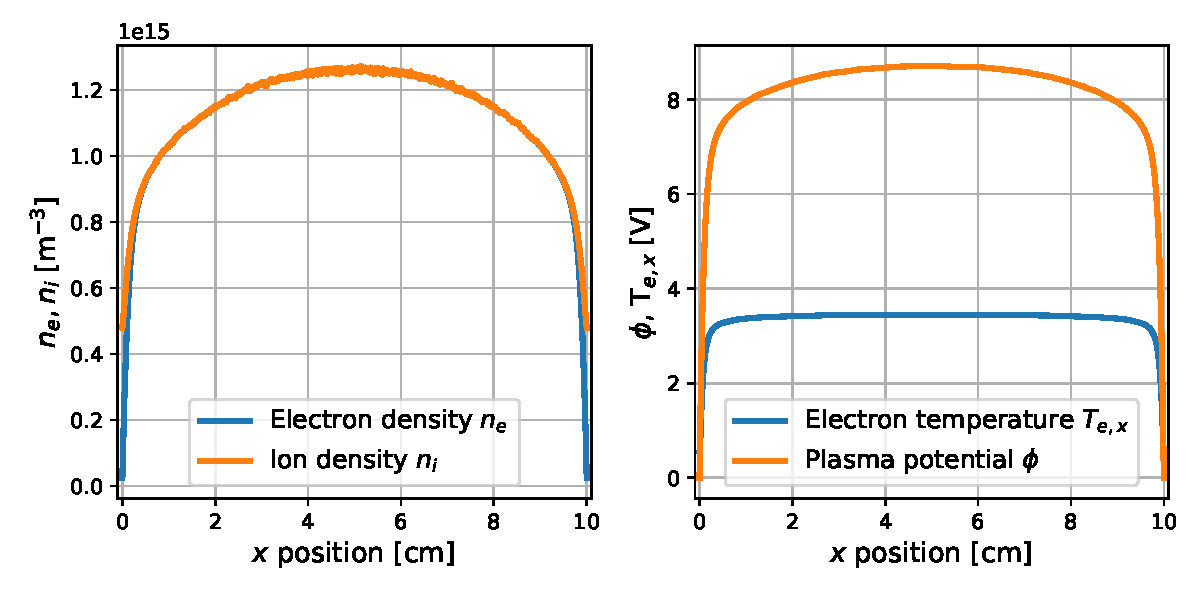
\includegraphics[width=0.9\textwidth]{ICP_results.pdf}
    \caption{Results of the PIC simulation for the self-consistent model, using RF inductive heating.}
    \label{fig-icpresults}
  \end{figure}

  \Cref{fig-icpresults} presents the simulation results for the electron density, plasma potential and electron temperature using the parameters of \Cref{tab-PIC2}.
  We can see that the different variables (density, electron temperature and the plasma potential) are not much affected compared to the results of \cref{sec-1DPIC}.

  \begin{figure}[!htbp]
    \centering
    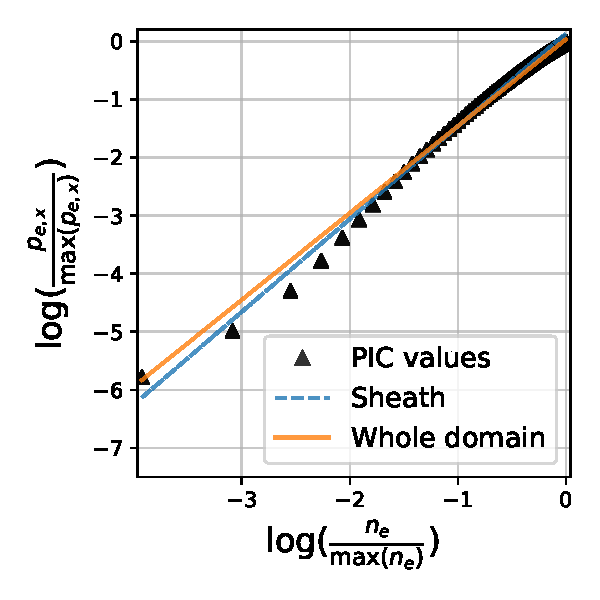
\includegraphics[width=\defaultwidth]{ICP_polyfit2.pdf}
    \caption{Estimation of the polytropic index in the sheath and in the whole domain in the PIC simulation using the self-consistent model.}
    \label{fig-icpfit}
  \end{figure}

  \Cref{fig-icpfit} presents the electron pressure as a function of the electron density measured in the simulation in log scale.
  We see that the trend is not purely linear. Hence, the linear regression used in order to obtain the polytropic index is conducted twice\string:
  \begin{itemize}
    \item In the whole domain\string: $\gamma=1.5$
    \item Only in the sheath\string: $\gamma=1.6$
  \end{itemize}
  The linear relation conducted of the whole domain is less precise than for the simulation result of \cref{sec-1DPIC} ($R^2=0.992$).
  However, we can see that the linear relation still describes quite well the electron evolution in the sheath.
  The polytropic indexes obtained with the self-consistent model are close to the simulation of \cref{sec-1DPIC} at the same pressure.

  \begin{figure}[!htbp]
    \centering
    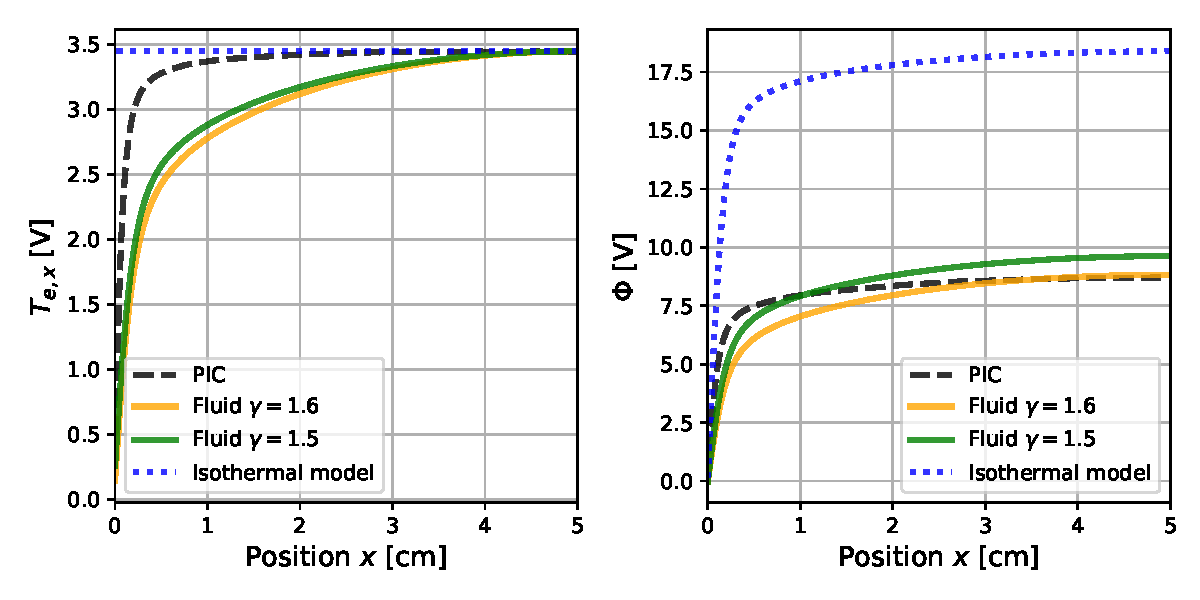
\includegraphics[width = 0.9\textwidth]{FluidComparisonICP.pdf}
    \caption{Comparison of the electron temperature and plasma potential measured in the PIC simulation with the prediction of the fluid model with $\gamma = 1.5$ (average index in the domain) and $\gamma=1.6$ (index in the sheath).}
    \label{fig-comp2}
  \end{figure}

  \Cref{fig-comp2} shows the comparison of the electron temperature and the plasma potential in the PIC simulation using the self-consistent model with the prediction of the fluid model of \cref{sec-fluid}.
  We can see that the agreement between the PIC results and the fluid models is less satisfactory than in \cref{fig-comp} when using the model unphysical plasma source, but it is still significantly better than the isothermal model.
  Hence, even with a self-consistent heating and ionization in the plasma, the polytropic model stands as a better model for the sheath and the pre-sheaths.

% !TEX root=/home/tavant/these/manuscript/src/manuscript.tex

\section{Monte Carlo computation of the EVDF}
\label{sec-MCM}
  
  The \ac{1D} \ac{PIC} simulations were computed faster than the \ac{2D} simulations, as the latter needed around a week to compute $10\,\micro\second$ on 360 CPUs, while the former needed only a few days on 64 CPUs to compute $20\,\micro\second$ of physical time.
  However, they still took a rather long time, especially when compared to fluid models that can be solve from under one second to around one day on a single core, depending on the hypotheses used.
  
  We have seen that the the polytropic index depends on several conditions, as the background pressure (see \cref{fig-p}) but also the densities, sizes, heating mechanism, and so on.
  We have seen in \cref{sec-fluid} that the only value of the polytropic index $\gamma$ is enough to describe the \ac{PIC} simulation.
  As the value of $\gamma$ depends on the \ac{EVDF}, we propose here a Monte Carlo approach that could be used in order to obtain the \ac{EVDF} faster that a \ac{PIC} simulation.
  A possible application would be similar to \citet{kushner1983}, where the author uses a small population of electrons (typically 300-500) and observes their evolutions in a given plasma potential.
  
  This method gets rid of the Poisson equation, which can take between 30\% and 50\% of the total simulation time.
  Hence, the Debye length does not have to be highly resolved any more for stability and numerical heating.
  However, we still need to resolve the sheath, which length is of the order of 5 Debye lengths \citep{chabert2014}.
  Consequently, a coarser mesh of cell size 5 times larger can be used.
  The condition on the time step is also reduced.
  This results in a much faster computation.

  \subsection{Description of the Monte Carlo approach}

    In order to validate the Monte Carlo approach, we use the converged simulation of the \ac{1D} \ac{PIC} model.
    We uses the potential, so the electric field, computed self-consistently in the \ac{PIC} simulation.
    The Monte Carlo is initialised with a uniform density of electrons.
    When an electron is collected at the wall, it is re-injected, similarly to the \ac{PIC} simulation.
    The electrons are pushed, and undergo collisions as described in \cref{sec-elements}.

    We validate the Monte Carlo computation by comparing the electron density, temperature and distribution function.
    \Cref{fig-EEPF_start_end} shows the expected EEPF obtained in the \ac{PIC} simulation with a background pressure of $P=1$\,mTorr.
    The maximum plasma potential, at the center of the domain, is $\max(\phi)=12.2\,\volt$.
    Is also shown in \cref{fig-EEPF_start_end} the EEPF at the beginning of the Monte Carlo computation, which corresponds to the Maxwellian distribution of temperature $\Te=5\,\volt$

    \begin{figure}[hbtp]
      \centering
      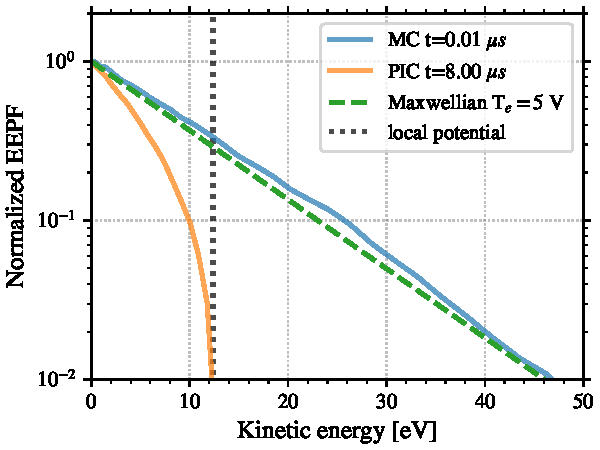
\includegraphics[width=\defaultwidth]{EEPF_PIC.pdf}
      \caption{Electron energy probability function obtained from (orange) the PIC simulation after convergence, and (blue) at the beginning of the Monte Carlo simulation. A Maxwellian distribution function at the $\Te{}_{,inj}$ and the local plasma potential are also given.}
      \label{fig-EEPF_start_end}
    \end{figure}

    \paragraph{Time scales \\}
    The electrons collected at the wall have a kinetic energy at least equal to the potential drop to the wall $\ek = e \dphi$, which corresponds in our case to a limit velocity of $v_{\rm lim} = \sn{1.5}{6} \,\meter\per\second$.
    Hence, the limit time of flight between the two boundaries is
    \[ T_{\rm flight} = \frac{L}{v_{\rm lim}} = 0.068 \,\micro\second  \]

    \vspace{1em}
    The electron-neutral scattering frequency is computed for a background pressure of $0.13$\,bar (${100}$\,mTorr) at the temperature of $300\,\kelvin$, which corresponds to a neutral density of $${n_g = \sn{3.2}{21} \meter^{-3}}.$$
    For an electron temperature of $5\,\volt$, the thermal electron-neutral elastic scattering frequency is 
    \[ \nu_{\rm ela} = 205 \,\mega\hertz.  \] 

    However, at this high energy, electron-neutral scattering is not isotropic, but instead gives mostly small angles (forward scattering) \citep{vahedi1995}.
    Hence, a large number of collision is required.
    The resulting time scale corresponding of the electron-neutral scattering is of the order of 
    \[ T_{\rm ela} \simeq \frac{100}{\nu_{\rm ela}} = 0.4 \,\micro\second  \]
    
    \inlinenote{Here, 1/$\nu = 0.004$, I don"t know why it is that low, while the MC calculations takes much more time to thermalize... Maybe due to the Injection ? \\ Anne: En regardant les temps sur tes resultats apres, j'ai compris ce qui te posait probleme ici. Tu es sur que dans ton monte carlo, ta densité de neutres n'est pas trop faible?}

    \paragraph{Numerical artefacts \\}
    In PIC simulations, numerical parameters can induce numerical heating and thermalization \citep{lai2014}.
    The numerical heating has been studied in detail \citep{birdsall1991}.
    It is due to aliasing effects, and depends on the grid size, time step and number of particles per cell.
    The choice of these parameter leads to reduce the effect of the heating.

    The thermalization is the fact that the distribution of the particle tends toward a Maxwellian.
    It originates from fluctuations of the electric field due to the discretization of the particle.
    The first studies showed that the thermalization time $\tau_T$ depends on $N_D$ the number of (numerical) particles per Debye sphere \citep{dawson1964,montgomery1970}.
    The presence of collisions can affect $\tau_T$  \citep{turner2006,lai2014}.
    In \citet{turner2006}, the author observed the evolution of the thermalization time with $N_D$ as
    \begin{equation} \label{eq-taut}
      \tau_T = \frac{1}{\omega_{pe}} \frac{34.4}{N_D^{-2} + 28.0 N_D^{-1} \frac{\nu_m}{\omega_{pe}}}
    \end{equation}
    which gives in our condition a time-scale several orders of magnitude larger than the other time scales $T_{\rm ela}$ and $T_{\rm flight}$ .
    Hence, the effects of numerical parameters on the kinetics informations of the simulation are expected to be negligible.
    We confirmed it by doubling the number of particle per cell for one pressure condition.
    No observable impact has been detected.

  \subsection{Results of the Monte Carlo computation} \label{subsec-MCMresults}

    We measured the electron energy distribution function (EEDF) at $3\,\centi\meter$ from the left wall.
    \Cref{fig-zoom_init_Mc} shows the evolution of the EEDF at the very early moments of the simulation, from $t=0.01$ to $0.08\,\micro\second$.
    The energy of the electrons is oriented, meaning that the electrons with positive energy are coming from the wall, while the negative energy is used for the electrons going toward the wall.

    \begin{figure}[hbtp]
      \centering
      \begin{tabular}{cc}
        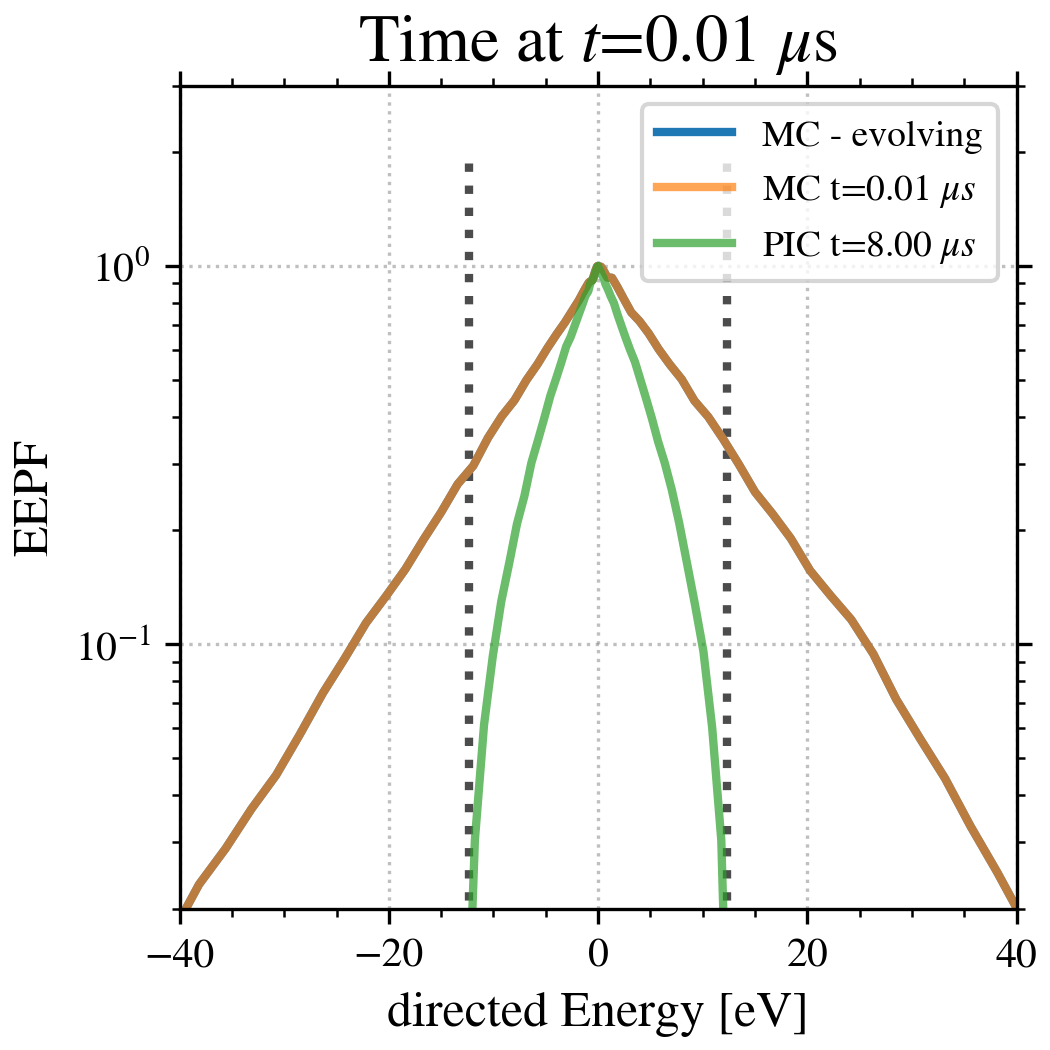
\includegraphics[width=0.4\textwidth]{MCC_EEDF/Heelo_1} &
        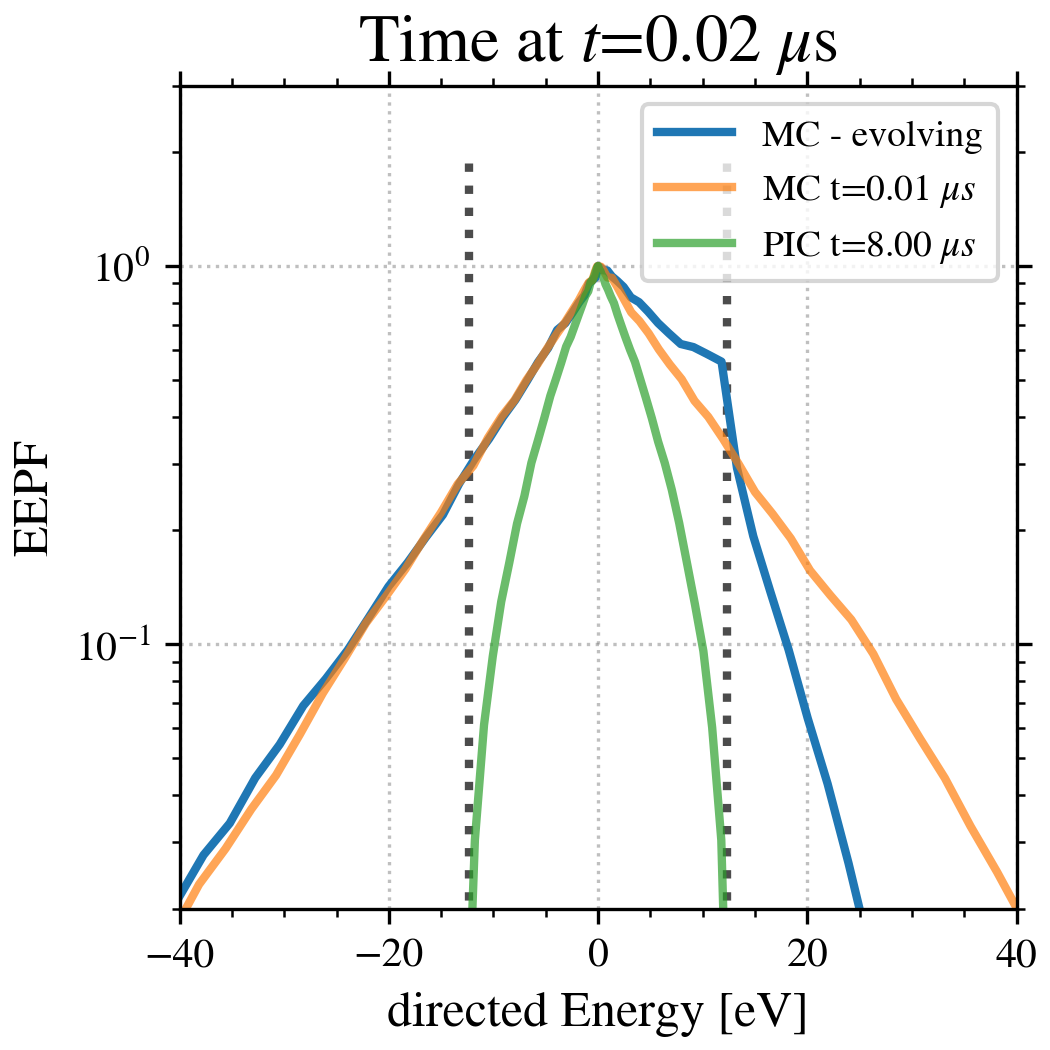
\includegraphics[width=0.4\textwidth]{MCC_EEDF/Heelo_2} \\
        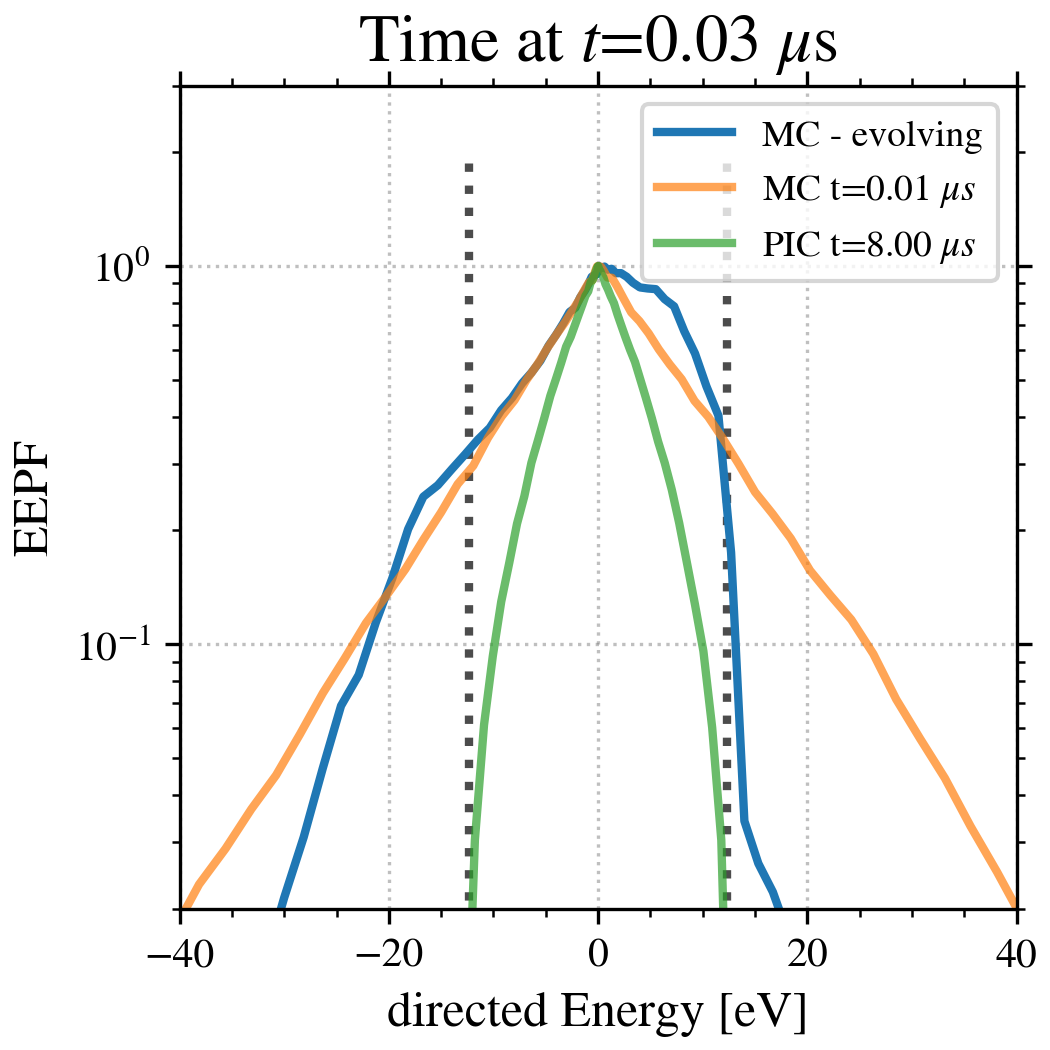
\includegraphics[width=0.4\textwidth]{MCC_EEDF/Heelo_3} &
        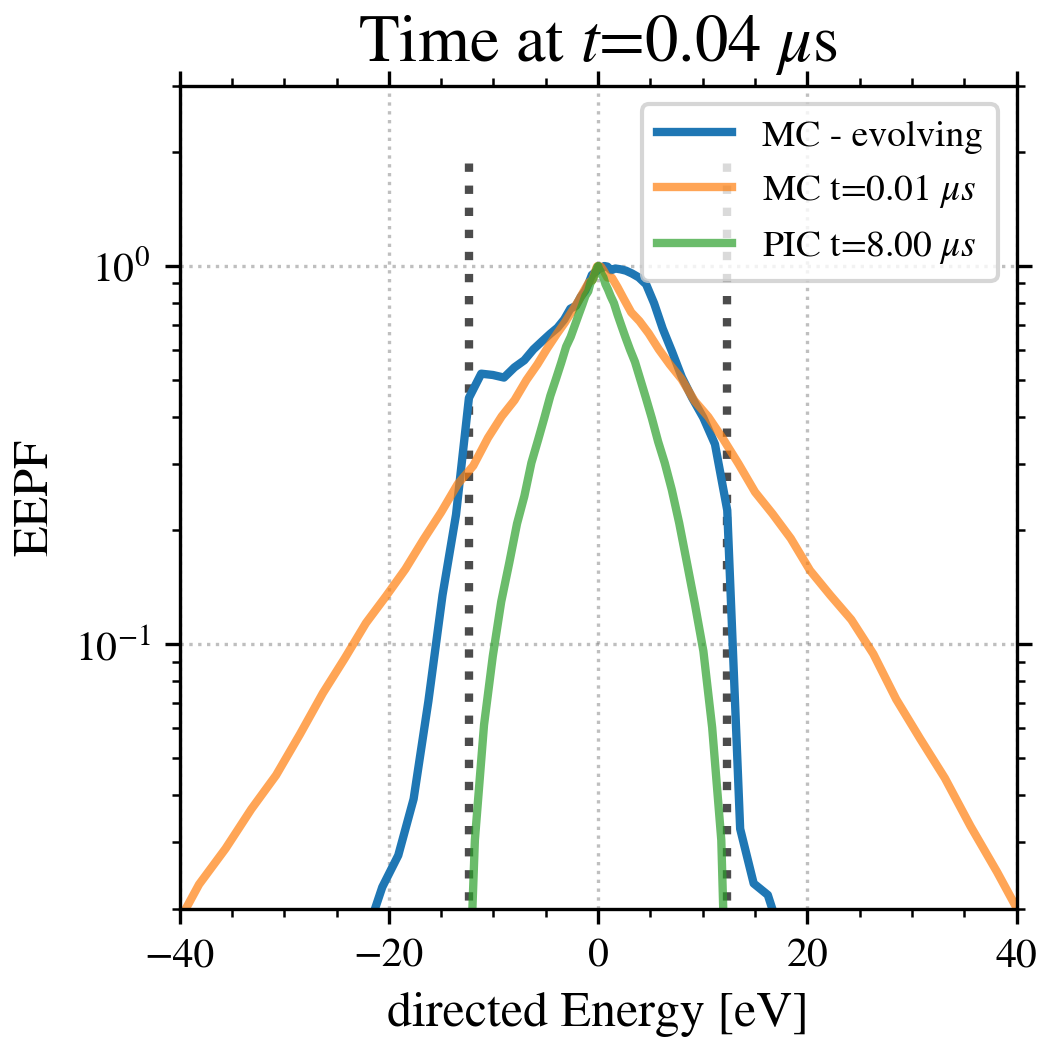
\includegraphics[width=0.4\textwidth]{MCC_EEDF/Heelo_4} \\
        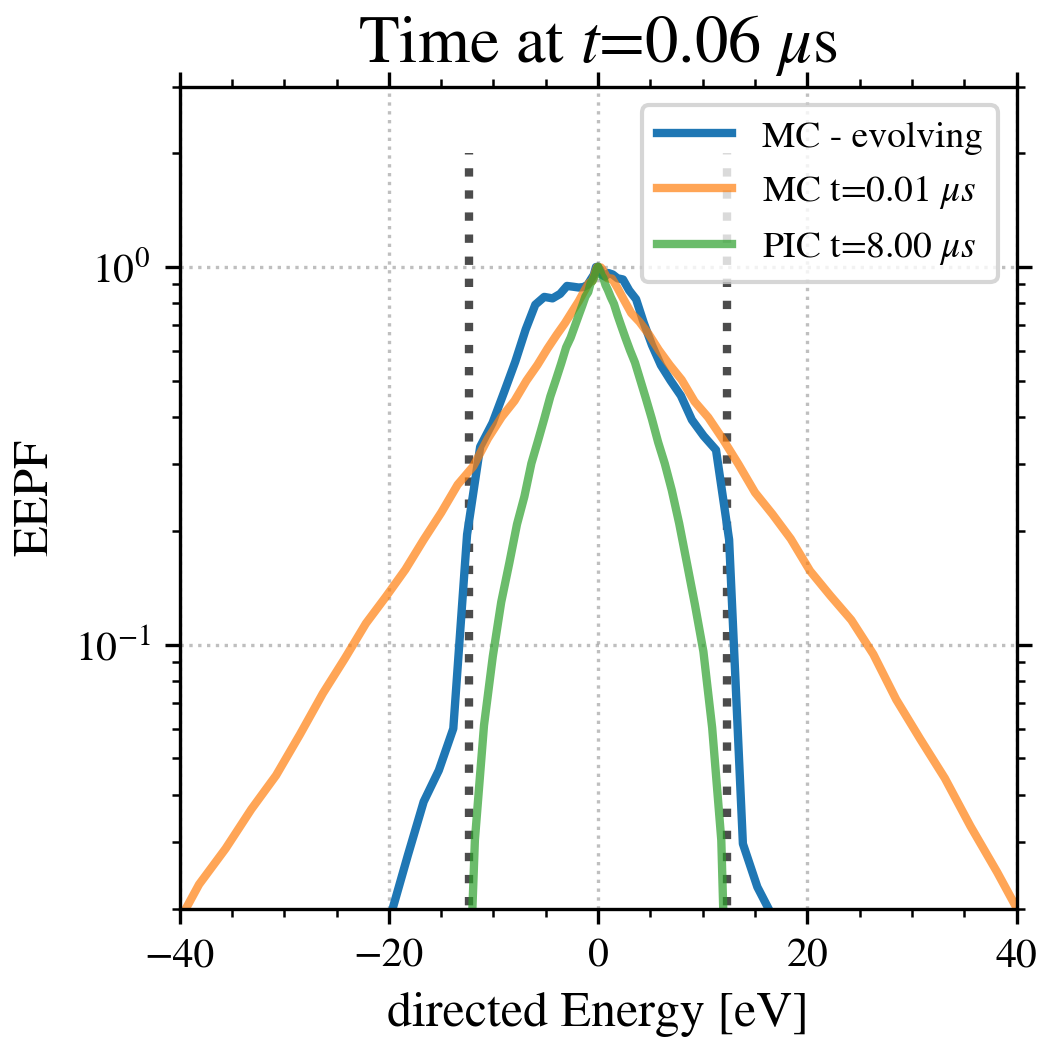
\includegraphics[width=0.4\textwidth]{MCC_EEDF/Heelo_6} &
        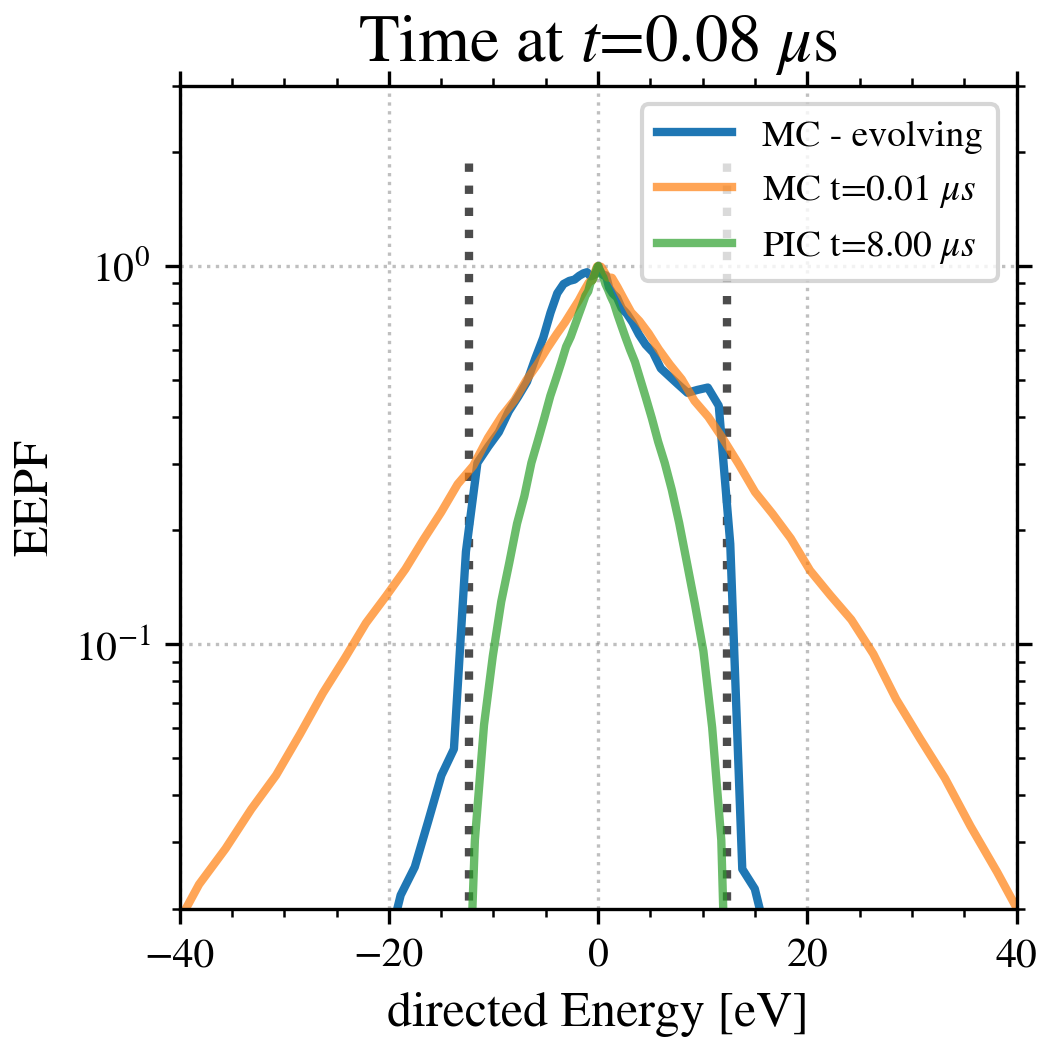
\includegraphics[width=0.4\textwidth]{MCC_EEDF/Heelo_8} \\
      \end{tabular}
      \caption{Evolution of the directed EEPF measured at $x=3\,\centi\meter$ from a wall. The positive energy is used for the electron going from the wall, while the negative energy represents the electrons moving toward the wall. The dotted line correspond to the local potential. Are overlaid (organge) the initial Maxwellian distribution and (green) the EEPF obtained at the end of the \ac{PIC} simulation. }
      \label{fig-zoom_init_Mc}
    \end{figure}

    Two phenomena can be seen in \cref{fig-zoom_init_Mc}.
    The first is the rapid decrease of the tail of the distribution function, for energies higher than the plasma potential.
    The tail for positive energy decreases faster than for negative energy, as the EEPF is measured closer to one wall than the other ($x=3\,\centi\meter$ against $L-x=7\,\centi\meter$).
    As expected, after $ T_{\rm flight}\simeq 0.07\,\micro\second$ the two tails are largely depleted, as they are one order of magnitude smaller than the Maxwellian EEPF.

    The second phenomena is the presence of waves in the velocity space that can be seen in the low energy populations.
    They are due to the plasma potential profiles.
    Indeed, the electrons are initialized with a uniform temperature, but their total energy depends on the local plasma potential. 

    \Cref{fig-zoom_Mc_later} shows the evolution of the EEDF over a longer time scale from $t=0.1$ to $2\,\micro\second$ compared to \cref{fig-zoom_init_Mc}.
    We can see the slow evolution of the low energy population from the initial, but slightly perturbed, Maxwellian distribution toward a distribution of smaller temperature.
    After $t=2\,\micro\second$, the EEPF of the Monte Carlo computation is fairly close to the \ac{PIC} EEPF.
    This is significantly longer than the estimated time scale of the elastic collisions ${T_{\rm ela}  = 0.4 \,\micro\second }$.
    \inlinenote{Why so ?? Est-ce que c'est parce que $T_{ela}$ est mal calculé ?}

    \begin{figure}[hbtp]
      \begin{tabular}{ccc}
        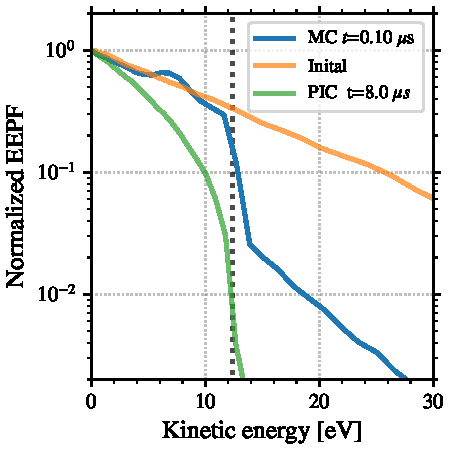
\includegraphics[width=0.3\textwidth]{MCC_EEDF/Heelo_1_10.pdf} &
        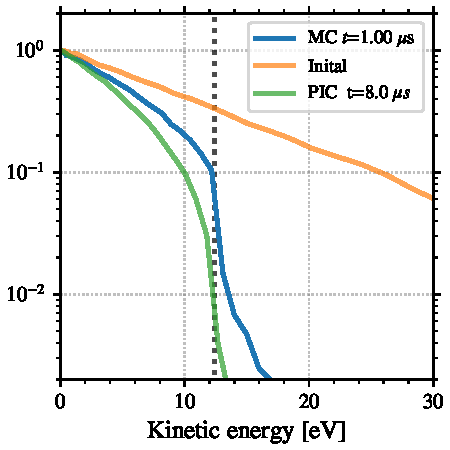
\includegraphics[width=0.3\textwidth]{MCC_EEDF/Heelo_1_100.pdf} &
        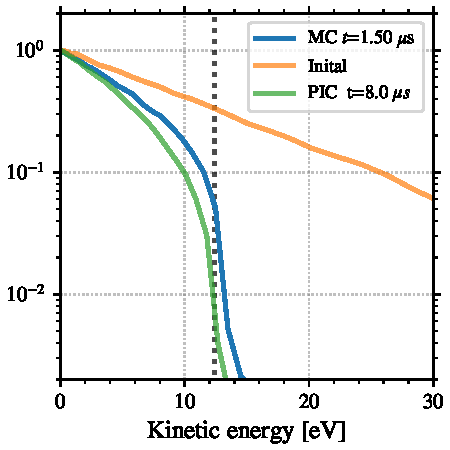
\includegraphics[width=0.3\textwidth]{MCC_EEDF/Heelo_1_150.pdf} \\
      \end{tabular}
      \caption{Evolution of the directed EEPF measured at $x=3\,\centi\meter$ from a wall. The dotted line corresponds to the local potential. Are overlaid (organge) the initial Maxwellian distribution and (green) the EEPF obtained at the end of the \ac{PIC} simulation. }
      \label{fig-zoom_Mc_later}
    \end{figure}

    \vspace{1em}
    This Monte Carlo investigation has shown that in the \ac{1D} model, the EEPF depends on the absorption at the wall but also the electron-neutral collisions.
    The final shape of the distribution is not simple, and is difficult to described and predict analytically.
    However, given the potential profile, the Monte Carlo computation reproduces the same distribution in a much shorter time compared to the \ac{PIC} simulation. 
    The obtained EEPF can then be used to determine the electron density and temperature evolution.
    This could be used to determine efficiently, and precisely, the electron polytropic coefficient.


% !TEX root=/home/tavant/these/manuscript/src/manuscript.tex

\section{Conclusion }
\label{sec-ch3conclusion}

Using the kinetic informations from the \ac{PIC} simulations, we have seen that the electrons are not Maxwellian, in contrast to the hypothesis of the usual models for plasma wall interactions.
The electron distribution function is affected by two phenomena\string:
\begin{itemize}
  \item the absorption of high energy electrons at the wall
  \item the electron-neutral scattering
\end{itemize}
\vspace{1em}
The absorption depletes rapidly the high energy tail of the EEPF for energies higher than the local plasma potential relative to the wall.
However, the low energy population is not affected by the wall

The collisions affect the electrons more slowly, by replenishing the high energy tail by scattering.
Indeed, in the directions parallel to the wall, the high energy tail is not depleted.
However, for large energies ($\ek > 10\,\volt$), the electron-neutral scattering angle is small \citep{vahedi1995}, hence the time scale over which the collisions impact the EEPF is much longer than the typical time between two collisions.

The electron trajectory in the discharge chamber is hence mostly collisionless.
We have successfully confirmed this by confronting the EEDF measurements to the 1D stationary Vlasov equation.
Following the work of \citet{zhang2016} on the collisionless evolution of non-Maxwellian electron through a potential drop, we have found that a polytropic closure for the electron describes very accurately the electron temperature evolution\string:
\begin{equation*} \label{eq-polyp2}
  \Te n_e^{1-\gamma} = cst, \text{ with $\gamma$ the polytropic index}
\end{equation*}

The polytropic state law for the electrons, when used in fluid model, allows to obtain the same densities and plasma potential as in the \ac{PIC} simulation.
This paves the way for a modified sheath model to compare to the \ac{2D} \ac{PIC} simulation of the \ac{HET} of \cref{ch-2}.

We have also seen in \cref{sec-realistic_1D} that the polytropic state law also stands when a self-consistent heating mechanism is used, even if the agreement is less satisfactory than in the other case.

In \cref{eq-polyp2}, the value of the polytropic index $\gamma$ depends on the shape of the \ac{EVDF}.
We showed in \cref{sec-MCM} that a Monte Carlo computation can be used in order to obtain the \ac{EVDF} for a given plasma potential profile and neutral pressure.
As the Monte Carlo approach does not need the Poisson equation to be solved, it produces the \ac{EVDF} much faster than a \ac{PIC} simulation.
Hence, we could couple the Monte Carlo calculation with a fluid model to accurately take into account the real shape of the \ac{EVDF} in the closure of terms in fluid models.



